
\section{Explainability: Where Does the Depth Disagree?}
\label{sec:explain}
Image metrics say how well a model re-renders the video, not where its depth is wrong. We now ask which per-pixel signals of a trained model rank its depth error against the stereo reference (Section~\ref{sec:unc_method}), and in which regions the error lies. All signals are computed from the model and its monocular prior before any stereo mask is applied. Table~\ref{tab:unc} summarises 2 sequences $\times$ 2 setups $\times$ 2 stereo references, each averaged over the test frames and three seeds.

\begin{table*}[t]
\caption{Which signal ranks the stereo-reference-relative depth error? Spearman $\rho$ between each per-pixel signal (computed from the model and its monocular prior only) and the per-frame scale-aligned AbsRel against SGBM stereo, and the share of the attainable ranking gain $G$ (Eq.~\ref{eq:gain}; ratio of the mean AURG to the mean random-order AUSE over 25 (P1) or 13 (P2\_5) test frames and three seeds; 100\,\% = oracle, 0\,\% = random). Strict: stereo pixels that pass a left--right consistency check. Best per column in bold.}
\label{tab:unc}
\centering\scriptsize
\setlength{\tabcolsep}{3.2pt}
\begin{tabular}{@{}lcccccccccccccccc@{}}
\toprule
 & \multicolumn{4}{c}{P1, FoV + DA} & \multicolumn{4}{c}{P1, ours} & \multicolumn{4}{c}{P2\_5, FoV + DA} & \multicolumn{4}{c}{P2\_5, ours (stereo-scaled)} \\
\cmidrule(lr){2-5}\cmidrule(lr){6-9}\cmidrule(lr){10-13}\cmidrule(lr){14-17}
 & \multicolumn{2}{c}{SGBM} & \multicolumn{2}{c}{strict} & \multicolumn{2}{c}{SGBM} & \multicolumn{2}{c}{strict} & \multicolumn{2}{c}{SGBM} & \multicolumn{2}{c}{strict} & \multicolumn{2}{c}{SGBM} & \multicolumn{2}{c}{strict} \\
Signal & $\rho$ & gain & $\rho$ & gain & $\rho$ & gain & $\rho$ & gain & $\rho$ & gain & $\rho$ & gain & $\rho$ & gain & $\rho$ & gain \\
\midrule
accumulated opacity (Endo-4DGS confidence) & -0.00 & -1 & 0.01 & -1 & 0.11 & 7 & 0.04 & 0 & 0.04 & -1 & 0.04 & 4 & 0.06 & 3 & 0.12 & 17 \\
ray depth spread & 0.20 & 20 & 0.21 & 10 & 0.15 & 5 & 0.09 & -4 & 0.07 & -13 & 0.04 & 12 & 0.14 & 16 & 0.18 & 26 \\
deformation magnitude & -0.06 & -2 & -0.01 & 6 & 0.04 & 9 & 0.03 & 18 & 0.10 & 7 & 0.07 & -1 & 0.25 & 39 & 0.17 & 26 \\
seed ensemble (3 seeds) & 0.24 & 31 & 0.22 & 37 & 0.15 & 8 & 0.06 & -10 & 0.29 & 29 & 0.21 & 25 & 0.20 & 31 & 0.21 & 24 \\
prior disagreement & 0.30 & 39 & \textbf{0.55} & \textbf{65} & \textbf{0.36} & \textbf{35} & \textbf{0.28} & \textbf{43} & \textbf{0.40} & \textbf{49} & \textbf{0.33} & \textbf{34} & \textbf{0.33} & \textbf{47} & \textbf{0.40} & \textbf{48} \\
combined (rank mean) & \textbf{0.39} & \textbf{49} & 0.52 & 63 & 0.30 & 31 & 0.21 & 27 & 0.36 & 41 & 0.28 & 33 & 0.30 & 42 & 0.35 & 43 \\
\bottomrule
\end{tabular}
\end{table*}


\begin{figure*}[t]
\centering
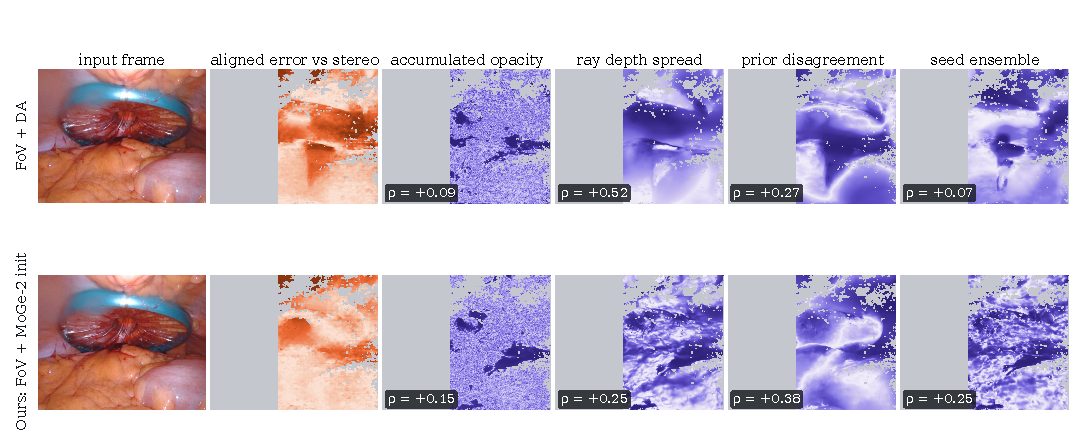
\includegraphics[width=\textwidth]{fig/expl_maps_p1.pdf}
\caption{Per-frame scale-aligned depth error against the stereo reference and four uncertainty signals for test frame 898 of P1 (seed 0). Uncertainty maps show per-frame percentile ranks (dark = most uncertain); $\rho$ is the Spearman correlation with the error on this frame. Grey: no stereo reference. Accumulated opacity is nearly unrelated to the error here, whereas prior disagreement and, for Depth-Anything, ray depth spread highlight the erroneous band below the instrument ring.}
\label{fig:explmaps}
\end{figure*}

\textbf{Accumulated opacity ranks depth errors weakly.} The accumulated opacity that Endo-4DGS uses as its confidence map reaches $\rho\le0.12$ and $-1$ to 17\,\% of the attainable ranking gain over all eight conditions, and is no better than a random ordering for both Depth-Anything models ($-1$ to 4\,\%). For our model it gives a small positive gain (0--17\,\%; Fig.~\ref{fig:sparse}), and the error in its most uncertain decile is 0.9--2.0$\times$ that of its least uncertain decile (Fig.~\ref{fig:calib}). This is consistent with how it is trained: the confidence loss uses global reductions (Section~\ref{sec:objective}), so $\hat{w}$ is not optimised as a per-pixel estimate of depth error. Our finding concerns this signal and loss, not learned uncertainty in general.

\textbf{Disagreement with the monocular prior is the strongest tested individual signal.} Measuring how far the rendered depth departs from the median-aligned prior of the same frame gives the highest $\rho$ and gain in seven of the eight conditions ($\rho=0.28$--$0.55$, 34--65\,\% of the attainable gain); the exception is FoV-corrected DA on P1 with the standard reference, where the rank combination is better (49 vs.\ 39\,\%). Pixels in its most uncertain decile have 1.9--4.8$\times$ the error of those in its least uncertain decile. With the strict reference its gain increases in three of the four settings, so it persists after filtering some stereo mismatches; this does not exclude errors shared by the reconstruction and the stereo reference. The signal is relative: it ranks pixels within a frame but does not provide an absolute reliability threshold. A plausible reason for its strength is that the reconstruction's depth largely inherits the prior's (Table~\ref{tab:priors}), so where training pulls the depth away from the prior, one of the two is likely wrong. The seed ensemble is a reasonable second for Depth-Anything (25--37\,\%) but inconsistent for MoGe-2 initialisation, whose seeds agree closely ($-10$ to 31\,\%). Ray depth spread is inconsistent ($-13$ to 26\,\%), and deformation magnitude is informative mainly on the static-camera sequence (26--39\,\% for ours on P2\_5), where apparent motion reflects tissue motion alone. The rank combination does not improve on prior disagreement elsewhere.

\begin{figure}[t]
\centering
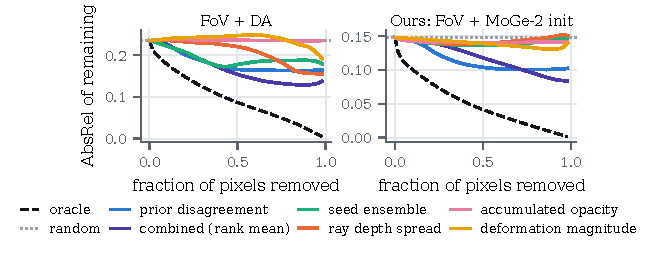
\includegraphics[width=\columnwidth]{fig/expl_sparsification_p1.pdf}
\caption{Sparsification curves on P1: mean scale-aligned AbsRel of the pixels that remain after removing the most uncertain fraction. Curves below the random line rank error; the dashed oracle removes pixels by their true error.}
\label{fig:sparse}
\end{figure}

\begin{figure}[t]
\centering
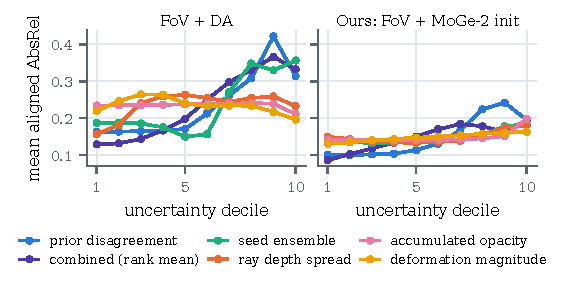
\includegraphics[width=\columnwidth]{fig/expl_calibration_p1.pdf}
\caption{Error by uncertainty decile on P1, a ranking diagnostic (not a calibration of predicted error magnitudes). A useful signal rises from left to right.}
\label{fig:calib}
\end{figure}

\textbf{Where the error lies.} Fig.~\ref{fig:regions} splits the error by disjoint region. On P1, depth edges (8.6\,\% of the scored pixels) have the highest per-pixel error for every model with the standard reference, but most of the total error lies on ordinary tissue: for our model, tissue carries 63\,\% of the summed error, depth edges 22\,\%, specular highlights 8\,\% and the ring 7\,\% (computed from per-frame error sums). Relative to FoV-corrected DA, MoGe-2 initialisation reduces the per-pixel error most on the ring ($-46$\,\%, 0.320 to 0.172) and on tissue ($-42$\,\%) and least at depth edges ($-15$\,\%). On P2\_5, which has no ring and smaller errors overall, tissue carries 84\,\% of the error, and the reduction relative to FoV-corrected DA is largest at depth edges ($-32$\,\%) and on tissue ($-29$\,\%) and smallest at specular highlights ($-16$\,\%). The strict reference changes which pixels are scored (on P1 specular pixels rise from 4.2 to 5.9\,\% and ring pixels fall from 5.6 to 3.7\,\% of the scored pixels) and raises the per-pixel error of specular and ring regions for all models, but tissue still carries 56\,\% of our error. The regions are defined by colour and stereo-gradient rules, so these numbers indicate trends rather than precise per-class errors.

\begin{figure}[t]
\centering
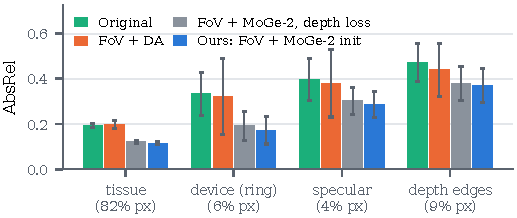
\includegraphics[width=\columnwidth]{fig/expl_regions_p1.pdf}\\[2pt]
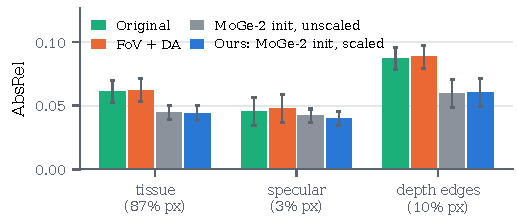
\includegraphics[width=\columnwidth]{fig/expl_regions_p25.pdf}
\caption{Per-frame scale-aligned AbsRel by disjoint region on P1 (top) and P2\_5 (bottom), mean $\pm$ s.d.\ over test frames and seeds; the share of scored pixels per region is given below each label.}
\label{fig:regions}
\end{figure}
